%!TEX root = ../thesis.tex
% ******************************* Thesis Appendix B ********************************

\chapter{Experimental Details} \label{appendix:experiments}

\section{Mpro assay} \label{appendix:mpro_assay}
The experimental procedure for measuring Mpro inhibition via Homogeneous Time Resolved Fluorescence (HTRF) assay is the same as that previously reported by COVID Moonshot\cite{Moonshot2022}, which is repeated below.

Dose response assays were performed in 12 point dilutions of 2-fold, typically beginning at 100\uM. Highly active compounds were repeated in a similar fashion at lower concentrations beginning at 10\uM or 1\uM. Reagents for Mpro assay were dispensed into the assay plate in 10$\mu$l volumes for a final volume of 20$\mu$L.

Final reaction concentrations were 20mM HEPES pH7.3, 1.0mM TCEP, 50mM NaCl, 0.01\% Tween-20, 10\% glycerol, 5nM Mpro, 37nM fluorogenic peptide sybstrate ([5-FAM]-AVLQSGFR-[Lys(Dabcyl)]-K-amide). Mpro was pre-incubated for 15 minutes at room temperature with compound before addition of substrate and ex/em filter set. Raw data was mapped and normalized to high (Protease with DMSO) and low (No Protease) controls using Genedata Screener software. Normalized data was then uploaded to CDD Vault (Collaborative Drug Discovery). Dose response curves were generated for IC50 using nonlinear regression with the Levenberg-Marquardt algorithm with minimum inhibition = 0\% and maximum inhibition = 100\%.

\section{OC43 antiviral assay} \label{appendix:oc43_assay}
A549 expressing H2B-mRuby were seeded in 384 well plates (4,000 cells per well) in DMEM+2\% FCS in a total volume of 30ul. One day later, 20ul of OC43 were added to the wells for a final MOI of 0.3. one hour after viral addition, the drug (or DMSO as control) was added to the cells. Drugs were added at a volume of 50nl, in a final dose range of 0.3-20mM. Cells were incubated at 33C, 5\% CO2 for 2 days, fixed with paraformaldehyde and stained for the presence of the viral nucleoprotein. Images were captured and quantified using the Incucyte machine and software. 3 biological repeated were performed.

\section{Model generated reaction schemes} \label{appendix:rxn_schemes}
\begin{figure}
    \centering
        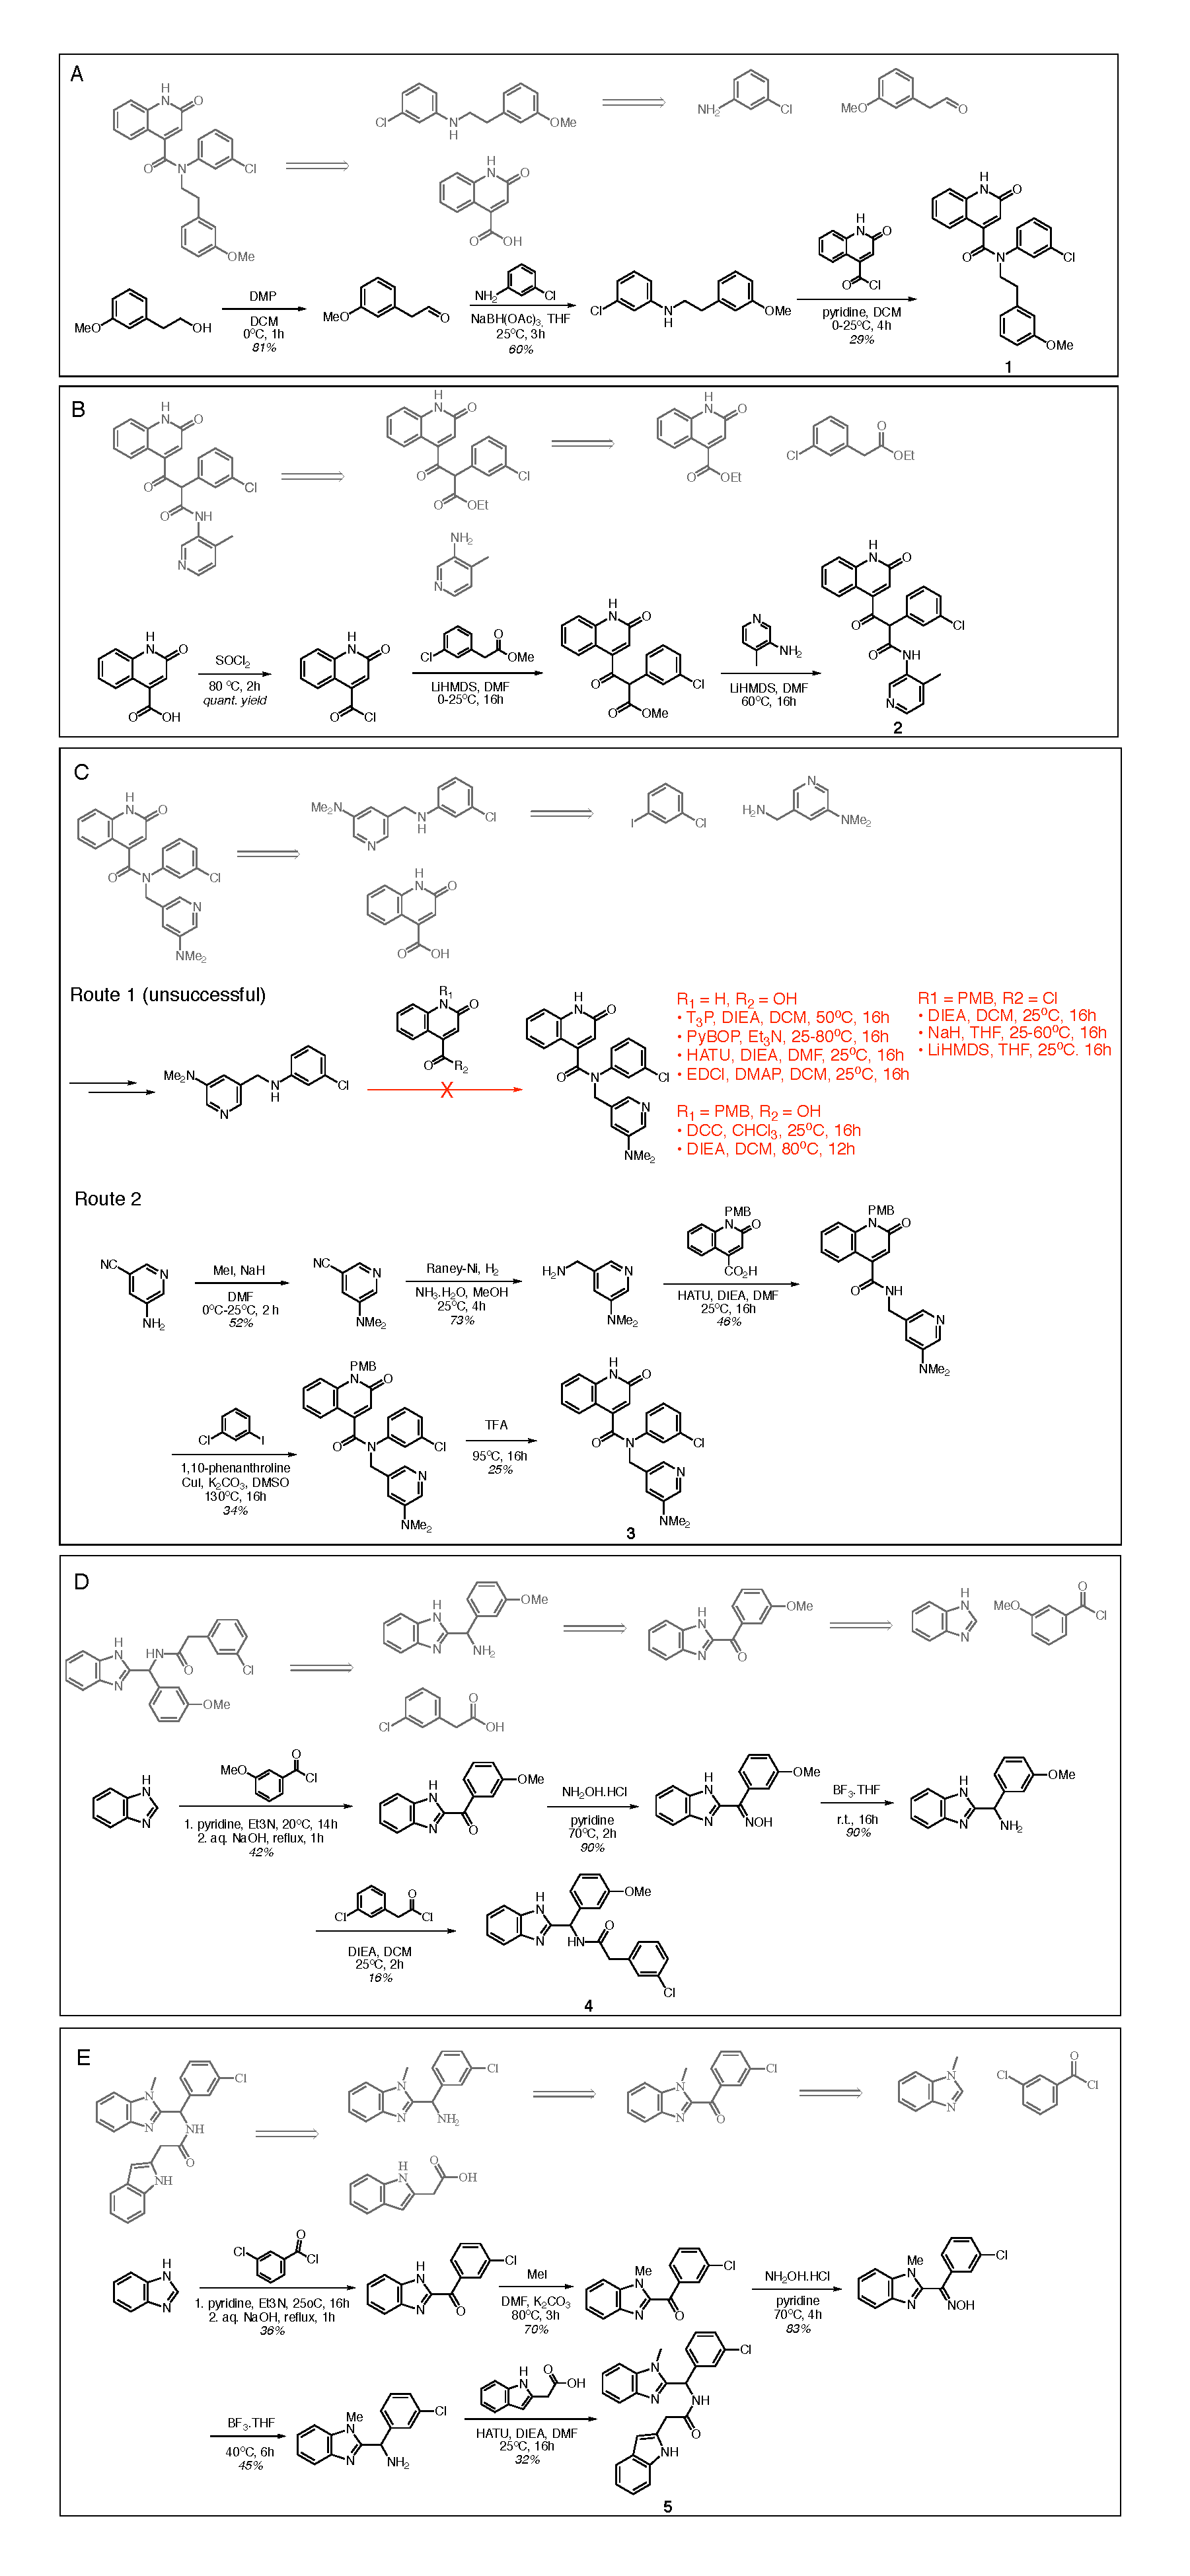
\includegraphics[width=0.6\textwidth]{Chapters/Ranking/Figs/rxn_schemes_full.pdf}
        \caption{Model generated synthetic schemes for compounds $\mathbf{1}$-$\mathbf{5}$. The synthesis schemes generated by our model (grey) and the experimental schemes (black).}
        \label{fig:appendix_synthesis_schemes}
\end{figure}

\section{Mac1 assay} \label{appendix:mac1_assay}
Inhibition of SARS-CoV-2 nsp3-Mac1 (aa residues 206–379 of nsp3) was assessed by the displacement of an ADP-ribose conjugated biotin peptide from His6-tagged protein using a HTRF-technology-based screening assay which was performed as previously described \cite{Schuller2021Mac1Frag}. Compounds were dispensed into ProxiPlate-384 Plus (PerkinElmer) assay plates using an Echo 525 liquid handler (Labcyte). Binding assays were conducted in a final volume of 16 $\mu$l with 12.5 nM SARS-CoV-2 nsp3-Mac1 protein, 400 nM peptide ARTK(Bio)QTARK(Aoa-RADP)S (Cambridge Peptides), 1:20000 Anti-His6-Eu3+ cryptate (HTRF donor, PerkinElmer) and 1:125 Streptavidin-XL665 (HTRF acceptor, PerkinElmer) in assay buffer (25 mM HEPES pH 7.0, 20 mM NaCl, 0.05\% bovine serum albumin and 0.05\% Tween-20). Assay reagents were dispensed manually into plates using a multichannel pipette while macrodomain protein and peptide were first dispensed and incubated for 30 min at room temperature. This was followed by addition of the HTRF reagents and incubation at room temperature for 1 h. Fluorescence was measured using a PHERAstar microplate reader (BMG) using the HTRF module with dual emission protocol (A = excitation of 320 nm, emission of 665 nm, and B = excitation of 320 nm, emission of 620 nm). Raw data were processed to give an HTRF ratio (channel A/B $\times$ 10,000), which was used to generate IC50 curves. The IC50 values were determined by nonlinear regression using GraphPad Prism v.9 (GraphPad Software, CA, USA).

\section{Crystallographic screening on SARS-CoV-2 nsp3-Mac1} \label{appendix:mac1_crystallography}
Crystallographic screening of compounds was performed using Mac1 crystals grown in the P43 space group, following the previously described protocol (PMID: 33853786). Compounds synthesized by Enamine/WuXi were prepared in DMSO to 100 mM and were added to crystallization drops using an Echo 650 liquid handler (Labcyte) (PMID: 28291760). Crystals were soaked at either 10 or 20 mM for 2-4.5 hours, before being vitrified in liquid nitrogen using a Nanuq cryocooling device (Mitegen). Soak times and concentrations are listed in Table S1. Diffraction data were collected at beamlines 12-1 and 12-2 of the Stanford Synchrotron Radiation Lightsource (SSRL). The data collection strategy and statistics are listed in Table S1. Compound binding was detected using the PanDDA algorithm (PMID: 28436492) as described previously (PMID: 35794891). PanDDA was initially run using a background map calculated with 34 datasets collected from crystals soaked only in DMSO (annotated as dmso\_34 in Table S1). PanDDA was rerun with a background map calculated using two sets of 35 datasets where no compound binding was detected (annotated as either ssrl\_1 or ssrl\_2 in Table S1). This procedure led to the identification of an additional nine hits (Table S1). 

Compounds were modeled into PanDDA event maps using COOT (PMID: 20383002) with coordinates and restraints generated by phenix.elbow from SMILES strings (PMID: 19770504). Duplicate soaks were performed for most compounds: where the same compound was identified in multiple datasets, the highest occupancy compound was modeled. Both the compound-bound and compound-free coordinates were refined together as a multi-state model following the protocol described previously (PMID: 28436492). Compound occupancy was set based on the background density correction (BDC) value (PMID: 28436492). Refinement statistics are presented in Table S1. Coordinates and structure factor amplitudes have been deposited in the protein data bank (PDB) with the group deposition code G\_1002254. PanDDA input and output files have been uploaded to Zenodo (DOI: 10.5281/zenodo.7231822), and the raw diffraction images are available at https://proteindiffraction.org/.

\section{High-Throuhput Amide Coupling} \label{appendix:amide_coupling}
The amide library was made by reacting the carboxylic acid under the optimized reaction conditions (2 eq. amine; 2 eq. EDC; 2 eq. HOAt; 5 eq. DIPEA; DMSO; RT; 24h) with 300 amines (202 aromatics, 49 primary, and 49 secondary aliphatic amines). For library production, we used Echo LDV plates and an Echo 555 acoustic dispenser for liquid handling. Plate copies were made after diluting the reaction mixture with 4 μL DMSO. For yield estimation, 1 μL of the diluted library was transferred to an LC/MS-ready 384-well plate, followed by dilution with 20\% ACN in water to the final volume of 50 μL. The desired product was identified in 60\% of wells.